\documentclass[a4paper]{article}
\usepackage{graphicx} %Required for diagrams
\usepackage[bookmarks=true]{hyperref}
\usepackage{bookmark}%Required to do pdf bookmarking
\usepackage[margin=1.2in]{geometry}
\usepackage{float}
\usepackage{caption}
\usepackage{hyperref}%Required for referencing website pages
\usepackage[english]{babel}

\usepackage{graphicx}
\usepackage{dcolumn}
\usepackage[table]{xcolor}

\title{User Manual}
\author{Baobab Team}

\begin{document}
\newpage

\begin{titlepage}

\begin{center}


\includegraphics[width=400px]{pictures/logo.jpg}
\vspace{0.5 cm}
\begin{flushright} \large
\begin{tabular}{lr}
\vspace{1 cm}
\LARGE\textbf{Document:}Sprint Report 6\\

\vspace{1 cm}
\LARGE\textbf{Project:} Group Chat For Linphone (Agile DO-178)\\
\vspace{1 cm}
\LARGE\textbf{Advisor:} Kobus Coetzee\\
\vspace{1 cm}
\LARGE\textbf{Sponsors:} Nanoteq \& Department of Computer Science, UP\\
\vspace{1 cm}
\LARGE\textbf{Date: }\today\\
\end{tabular}
\end{flushright}

\centering 
\includegraphics[width=350px]{pictures/Team.jpg}

Patience Mtsweni, Lerato Molokomme, Tsepo Ntsaba, Mpedi Mello, Lutfiyya Razak, Ephiphania Munava\\


\end{center}
\end{titlepage}
\newpage

\section{Introduction}
The user manual specified below provides instruction for the users of Linphone group chat on what and how to use the system therefore it specifically focuses on system configuration, installation, using the system and troubleshooting.

\section{General Information}


\subsection{Project Details}

%Lerato edit here - System name and the names and/or affiliation of all stakeholders.
\setlength{\arrayrulewidth}{0.5mm}
\setlength{\tabcolsep}{12pt}
\renewcommand{\arraystretch}{2} 
\begin{tabular}{ |p{3cm}|p{3cm}|p{3cm}|  }
\hline
\rowcolor{lightgray}\multicolumn{2}{|c|}{System name affiliation of all stakeholders} \\
\hline
System name & Linphone Group Chat \\
\hline
Stakeholder & Kobus Coetzee \\
\hline
Scrum master  & Potego Mello\\ \hline 
Client representative  & Patience Mtsweni\\ \hline 
UX developer  & Lutfiyya Razak and Lerato Molokomme\\ \hline 
Backend developer  & Ephiphania Munava and Potego Mello\\ \hline 
Crypto developer  & Tsepo Ntsaba \\ \hline 
CI / CD support  & Patience Mtsweni \\ 
\hline
\end{tabular}

\subsection{System Overview}


Linphone is the leading open source implementation of Voice over IP (VoIP) and Instant Messaging (IM) functionalities. This particular release of Linphone runs on the android platform and aims to extend Linphone's instant messaging capabilities by including group chat and improving it's user interface. This application also seeks to secure the group chat, so that the user's communication is not intercepted by third parties. The application provides the end-user with group chat functionalities found in closed source competitors like WhatsApp.\\

Now users are able to exchange messages in a conference like manner. In addition to exchaging text messages, multiple users are also now able to exchange pictures and voice notes in a single chat-room and the messages are distinguished according to the person who sent them. \\

There are two types of users levels for the group chat, namely administrator and standard users. Administrator users can do everything that the standard user can do, plus some additional capabilities. Only administrator users (initially the person who created the group) are able to add and remove members of the group, with the current capacity being 20 members per group.\\

Standard users are provided the functionality to remove themselves from the group if they no longer want to be part of that group. In the case that the person leaving the group is an administrator, then a random user should be selected from the remaining members to be the administrator but with this current release the group is deleted.\\

If all members leave the group, then it is destroyed and ceases to exist. The only other way to delete the group is via an administrator. The administrator is also allowed to remove individual members they feel should no longer be part of the group.

\subsection{System Configuration}

%Ephiphania Edit Here
\subsubsection{Equipment}
An Android phone is a smartphone that runs on Google's open-source Android operating system. There are a number of different manufacturers that make Android phones, namely HUAWEI, LG, ASUS, acer, Virgin mobile, Samsung, Motorola, Sony and many more.\\

\begin{center}
\begin{figure}[h]
\centering

\includegraphics[width=0.7\linewidth]{./pictures/android.jpg}
\caption{\label{fig:Agile}Android Phones.}
\end{figure}
\end{center}

\subsubsection{Network}
The linphone application requires registration to a SIP provider before you can operate it. The provider ensures that you have a SIP address which is a Uniform Resource Identifier also known as a URI which is represented in the form user@domain.tld. \\


\begin{center}
\begin{figure}[h]
\centering
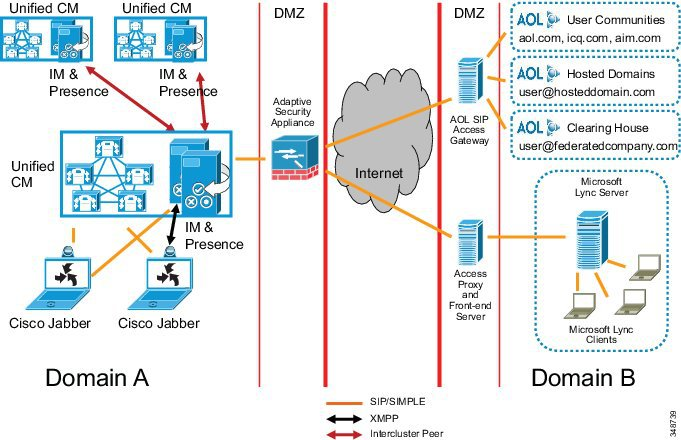
\includegraphics[width=0.5\linewidth]{./pictures/sip.jpg}
\caption{\label{fig:Agile}SIP Protocol.}
\end{figure}
\end{center}

Linphone.org hosts a free SIP service which allows users to make audio or video calls using SIP addresses under the domain sip.linphone.org. \\
When creating your sip address like sip:baobab@sip.linphone.org you simply use the form provided on http://www.linphone.org/free-sip-service.html and your friends can communicate with you by simply making use of the sip address.
\\
%\begin{center}
%\begin{figure}[h]
%\centering
%\includegraphics[width=0.4\linewidth]{./pictures/LinphoneSip.jpg}
%\caption{\label{fig:Agile}Linphone SIP Registration.}
%\end{figure}
%\end{center}

All of the above describes configuration of the already existing Linphone application. This is not by mistake. The process used by the group chat to exchage messages is similar to that of private chats.
\\

All of the group capabilities are on the client side (code that sits purely on your Android device). Therefore, there is no extra configuration needed to accommodate the group chat functionality. We pride ourselves in making the transition into group chat easy and simple for the user.


\subsection{Installation}
\begin{itemize}
\item Turn on your Android Smartphone and open your favourite web browser.
\item In the address bar, type in \textbf{“http://thebaobabteam.github.io/linphone-android”} and press enter.
\item Download the file “Linphone-android.apk”.
\item Go to your phone settings and turn on the option to allow installation of non-Market applications (Unknown sources).
\item Run the downloaded file (linphone-android.apk) by clicking on it.
\item Confirm that you accept the Linphone application rights on the screen that will be appear on your Smartphone by tapping “Accept”. When the file installation is done tap “Open”.
\item Press “Agree” when the License Agreement appears on your screen to finalize the install and start Linphone for Android.
\end{itemize}

\subsection{Getting started}

\subsubsection{Registering on the network}
To get started with the system, you need to install Linphone Application onto your android phone. To do this refer to section(2.4), and follow the results as shown there.\\

Once you have Linphone installed, you should setup your sip account, which you will need to be able to use the system. For more details on what a SIP address is, refer to section (2.3.2).\\


\begin{itemize}
\item Click on the \textbf{settings} button on the bottom of the screen. Next click on  \textbf{Account Setup Assistant}.
\end{itemize}

\begin{figure}[h]
  \centering
  \begin{minipage}[h]{0.4\textwidth}
    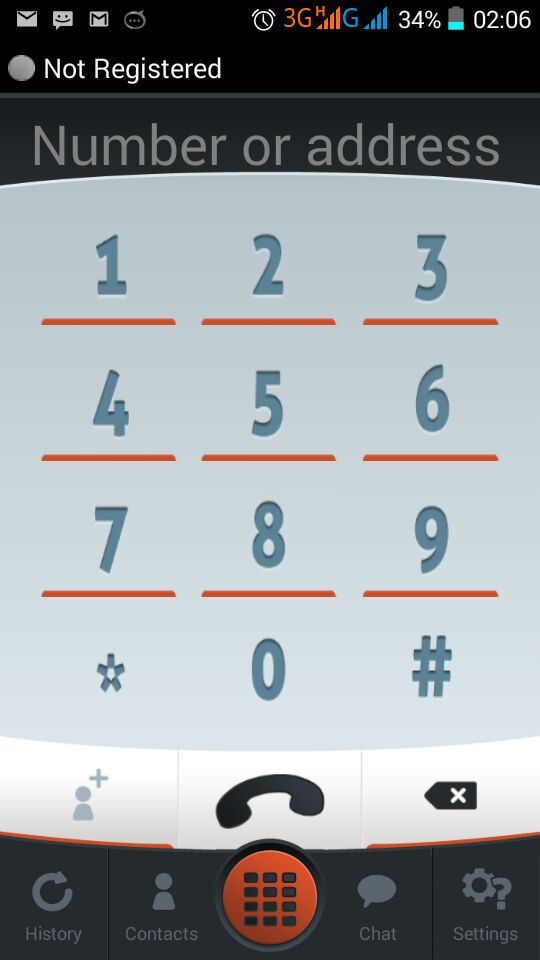
\includegraphics[width=40mm, scale=0.5]{pictures/home.png}
    \caption{Home Screen}
  \end{minipage}
  \hfill
  \begin{minipage}[h]{0.4\textwidth}
    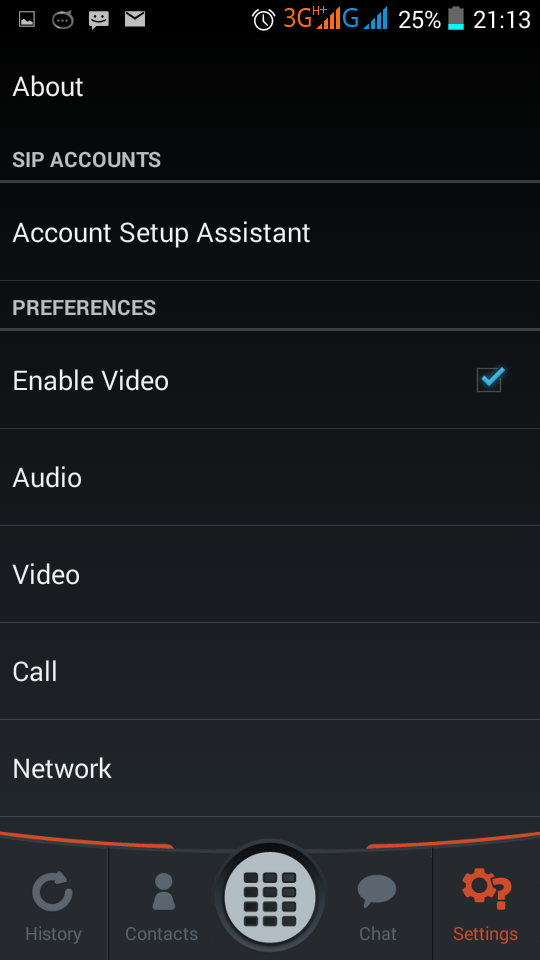
\includegraphics[width=40mm, scale=0.5]{pictures/settings.png}
    \caption{Settings Screen}
  \end{minipage}
\end{figure}

\begin{itemize}
\item Click on \textbf{Let's go}. Next, click on \textbf{Create account on linphone.org} then click \textbf{Create} . \\
\item Otherwise, if you already have a SIP or linphone.org account, click on their options and click \textbf{Apply} .
\end{itemize}

\begin{figure}[h]
  \centering
  \begin{minipage}[h]{0.4\textwidth}
    
\includegraphics[width=40mm, scale=0.5]{pictures/welcome.png}
    \caption{Account Setup Screen}
  \end{minipage}
  \hfill
  \begin{minipage}[h]{0.4\textwidth}
    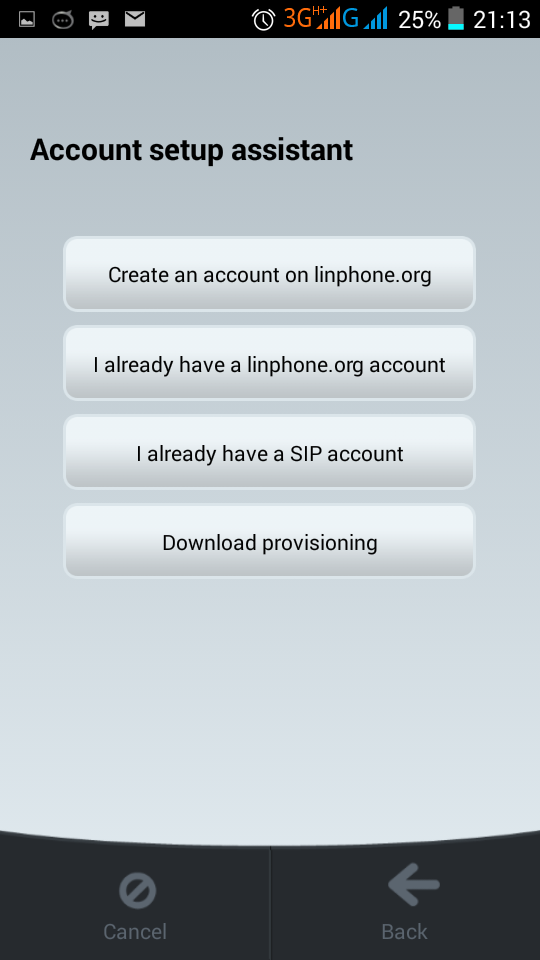
\includegraphics[width=40mm, scale=0.5]{pictures/options.png}
    \caption{Options Screen}
  \end{minipage}
\end{figure}


\newpage

\subsection{Using the system}
%Potego Edit Here

After successful installation and setup (sip account) of the linphone application, you should then see the following screen:

\begin{center}
\begin{figure}[H]
\centering

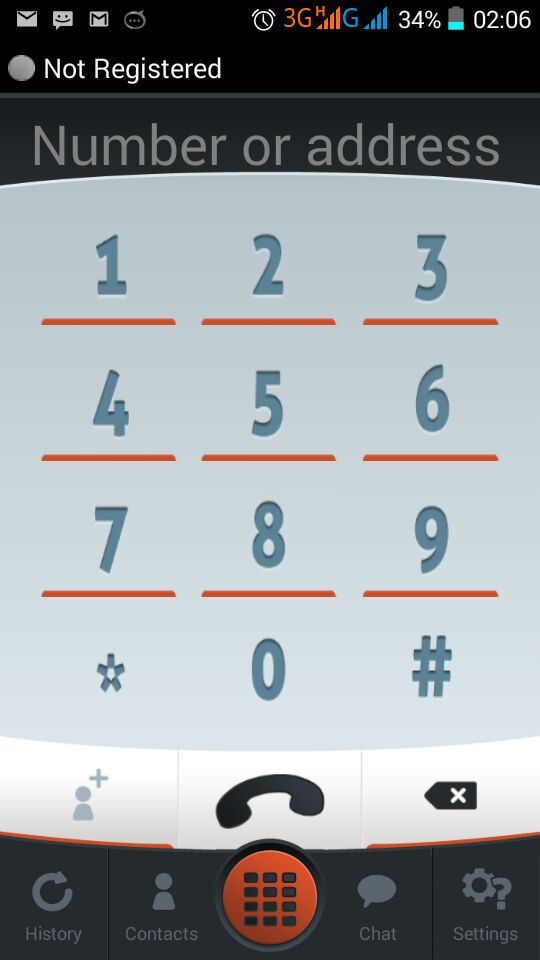
\includegraphics[width=0.4\linewidth]{pictures/home.png}

\caption{\label{fig:Screen1}Main Screen.}
\end{figure}
\end{center}

%
%To make call via VoIP (Voice over Internet Protocol), type in (where it's written "Number or address") the sip address or the phone number of the person you would like to contact and press the dial button like screen two:
%
%\begin{center}
%\begin{figure}[H]
%\centering
%
%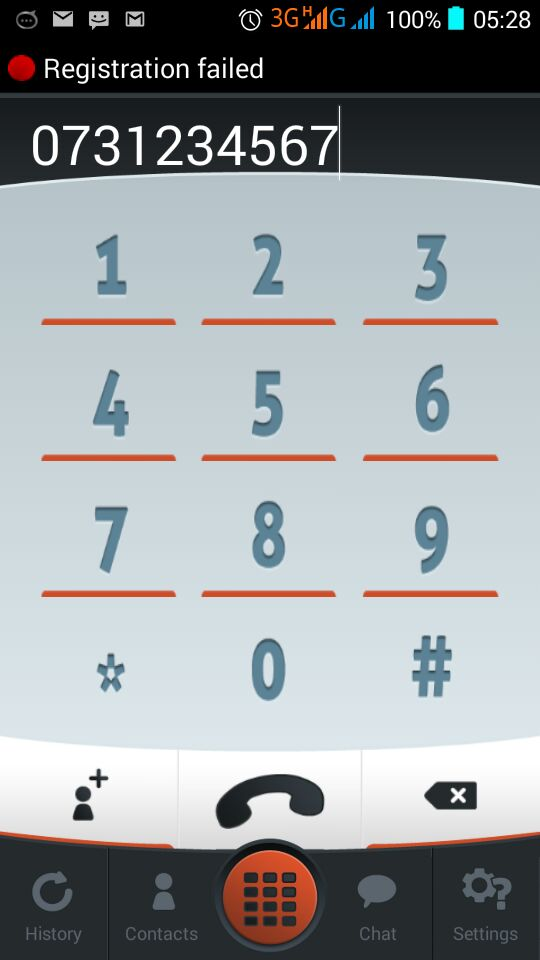
\includegraphics[width=0.4\linewidth]{pictures/Screenshot_2015-08-04-05-38-27.png}
%
%\caption{\label{fig:Screen2}Screen two.}
%\end{figure}
%\end{center}

To start chatting just click on the chat button in the menu at bottom of the screen. It will take you to the following screen:

\begin{center}
\begin{figure}[H]
\centering

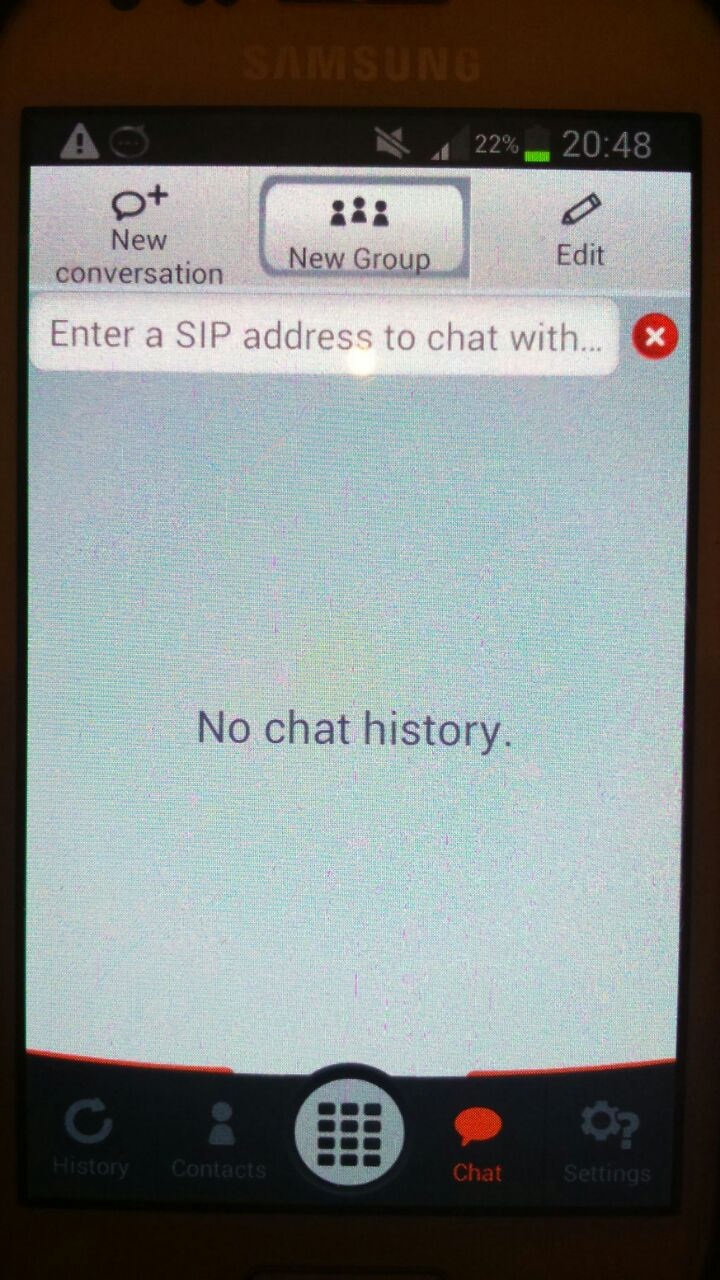
\includegraphics[width=0.4\linewidth]{pictures/s1.jpg}
\caption{\label{fig:Screen3}Screen three.}
\end{figure}
\end{center}

Now click on the "group chat" icon at the top left, second position which will then lead you to the create group chat screen which looks like the picture below in the following:
%
%\begin{center}
%\begin{figure}[H]
%\centering
%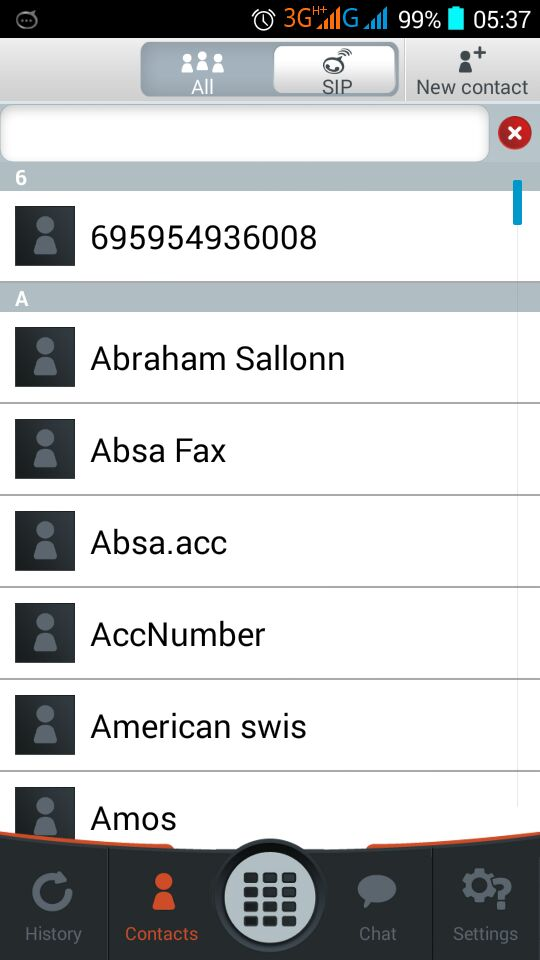
\includegraphics[width=0.4\linewidth]{pictures/Screenshot_2015-08-04-05-37-18.png}
%\caption{\label{fig:Screen4}Contact List.}
%\end{figure}
%\end{center}
%
Select a group picture either by taking a photo or selecting a picture from the gallery and press enter. Look at the following:

%%\begin{center}
%%\begin{figure}[H]
%%\centering
%%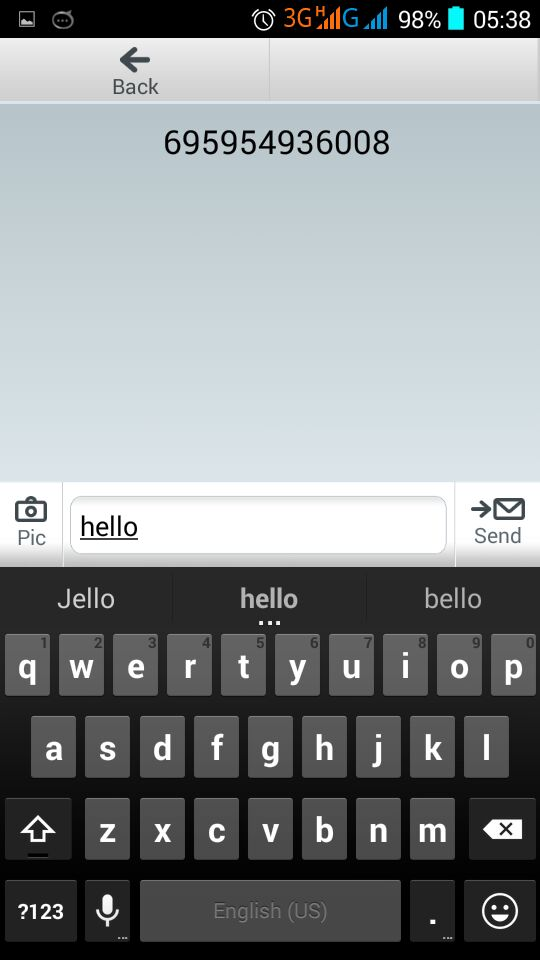
\includegraphics[width=0.4\linewidth]{pictures/Screenshot_2015-08-04-05-37-53.png}
%%\caption{\label{fig:Screen5}Chatroom.}
%%\end{figure}
%%\end{center}
%
%There is a small text box at the bottom of the chatroom that can be used to compose your messages and then when ready, you can click on the send button next to it to send the message to your peer. Like this:
%
%\begin{center}
%\begin{figure}[H]
%\centering
%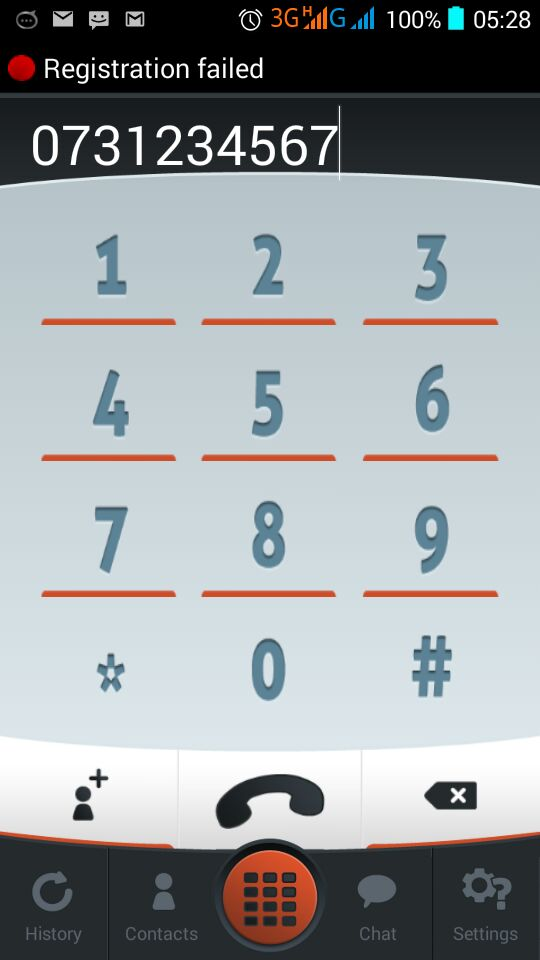
\includegraphics[width=0.4\linewidth]{pictures/Screenshot_2015-08-04-05-38-27.png}
%\caption{\label{fig:Screen6}Chatroom 2.}
%\end{figure}
%\end{center}
%
%To add new contacts via linphone just go back to the main screen and click on the contacts button. This will take you to the Contact list screen. At the to right position of that screen click on the new contact button and you will be led to the following screen:
%
%\begin{center}
%\begin{figure}[H]
%\centering
%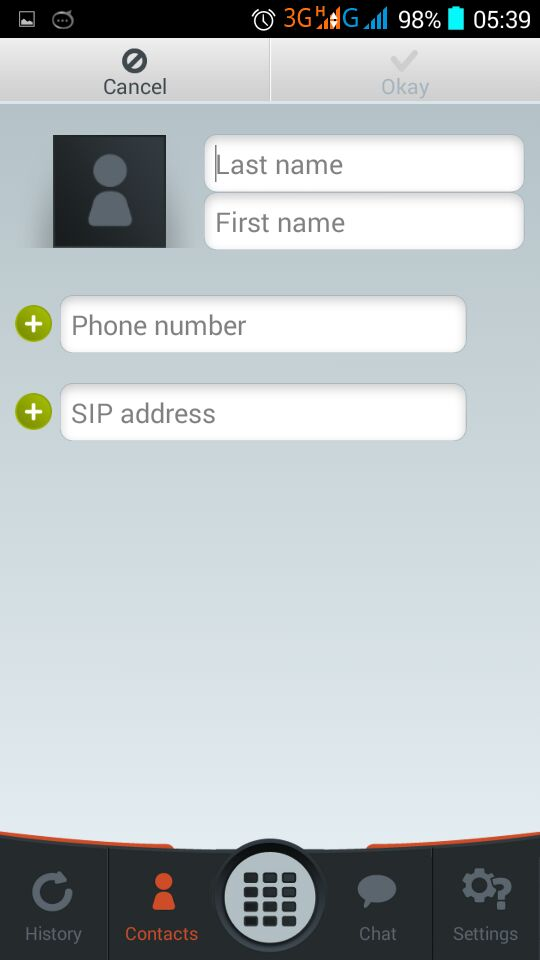
\includegraphics[width=0.4\linewidth]{pictures/Screenshot_2015-08-04-05-39-24.png}
%\caption{\label{fig:Screen7}Create New Contact.}
%\end{figure}
%\end{center}
%
%Now you can fill in the details required in the form and then click on Okay to save the new contact. Like so:
%
%\begin{center}
%\begin{figure}[H]
%\centering
%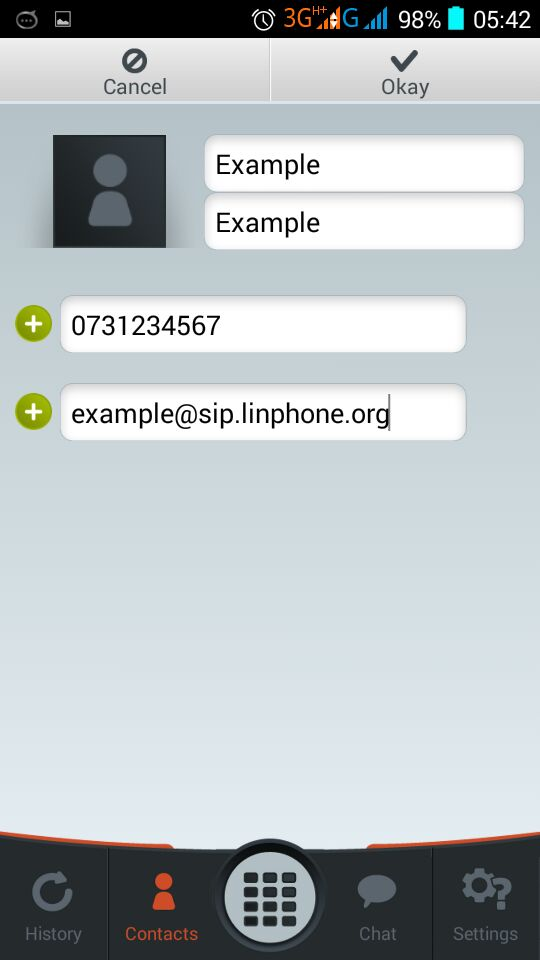
\includegraphics[width=0.4\linewidth]{pictures/Screenshot_2015-08-04-05-40-26.png}
%\caption{\label{fig:Screen8}Create New Contact with details.}
%\end{figure}
%\end{center}
%
%Your call logs can be found by going back to the main screen and then clicking on the History button at the bottom left screen menu. The log for outgoing and incoming calls are shown here:
%
%\begin{center}
%\begin{figure}[H]
%\centering
%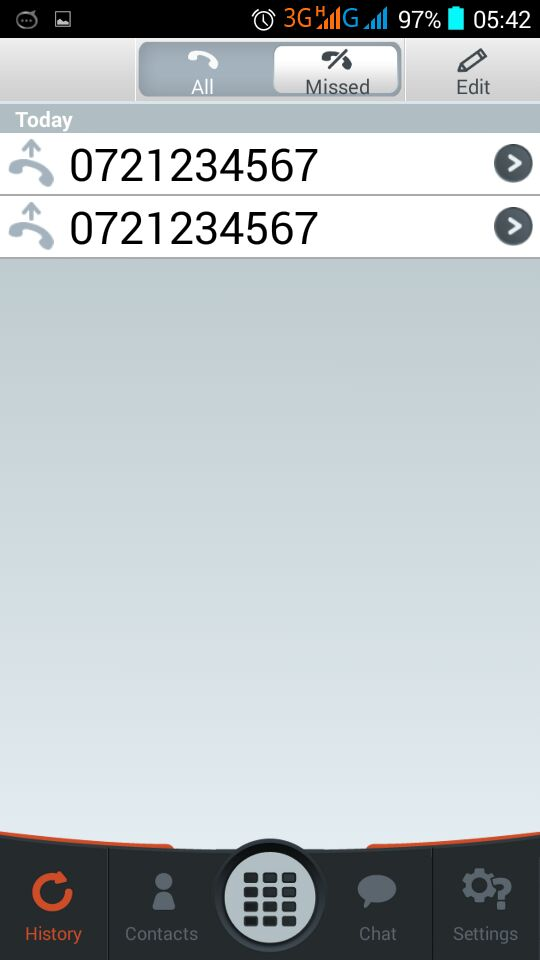
\includegraphics[width=0.4\linewidth]{pictures/Screenshot_2015-08-04-05-42-53.png}
%\caption{\label{fig:Screen9}Call Log History.}
%\end{figure}
%\end{center}

\newpage
\subsection{Troubleshooting}
\textbf{Troubleshooting, FAQ and Problems} \\

\textbf{Connection problems} \\
I try to phone to my friend <sip:toto@example.com>, but nothing happens, no ring, nothing
at all. \\
You must verify that linphone uses the network interface that connects you to the
internet (or to the network where calls should go). \\
Use the property box, section Network, to select the correct network interface.
In other case, the person you are contacting may be not reachable at the moment... \\

\textbf{Audio problems} \\
Linphone seems to connect to the remote sip url, it rings, but when the callee answers,
nothing happens and we can't hear each other. \\

Most people get problems because they don't choose the correct network interface
in the property box, section network. \\

In other cases, it will fail. \\
First rise up playback and recording level. \\
If the voice is sometines cutted, you can modify parameter RTP\->jitter \\
compensation in the property box to greater values to avoid this. But it increases the
delay transmission. \\

\textbf{FAQ}
How do I use Linphone Calling? \\
Linphone Calling lets you call your friends and family using Linphone for free, even if they're in another country. Currently, Linphone Calling is available on Android. \\
Linphone Calling uses your phone's Internet connection rather than your cellular plan's voice minutes. Data charges may apply.
Please note: you can't access 10111 and other emergency service numbers through Linphone. You must make alternative communication arrangements to make emergency calls. \\

\textbf{Bugs reporting and suggestions} \\
First go to linphone's home page at http://www.linphone.org to check if you have the
latest version of linphone. \\

\end{document}

